\subsection{Our improved Dynamic Frontier (DF) approach for Real-world Dynamic Graphs}
\label{sec:frontier}

If a batch update $\Delta^{t-} \cup \Delta^{t+}$ is small compared to the total number of edges $|E|$, then it is expected that the ranks of only a few vertices change. Our proposed Dynamic Frontier approach incorporates this aspect, and identifies affected vertices via an incremental process. This allows it to avoid unnecessary computation, since ranks of vertices far for the updated region of the graph cannot have a change in their ranks until the ranks of its immediate in-neighbors change. In addition, we avoid marking the neighbors of a vertex as affected, if the change in rank of the vertex is small enough and is likely to have minimal effect on the ranks of its neighbors.


\subsubsection{Explanation of the approach}
\label{sec:frontier-explanation}

Consider a batch update consisting of edge deletions $(u, v) \in \Delta^{t-}$ and insertions $(u, v) \in \Delta^{t+}$. We first initialize the rank of each vertex to that obtained in the previous snapshot of the graph.

\begin{figure*}[hbtp]
  \centering
  \subfigure[Initial graph]{
    \label{fig:about-frontier-df1}
    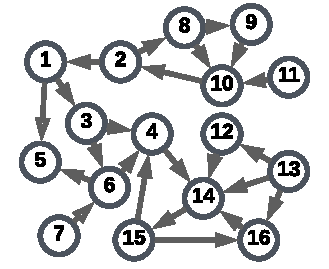
\includegraphics[width=0.23\linewidth]{out/about-frontier-11.pdf}
  }
  \subfigure[Marking initial affected vertices (DF)]{
    \label{fig:about-frontier-df2}
    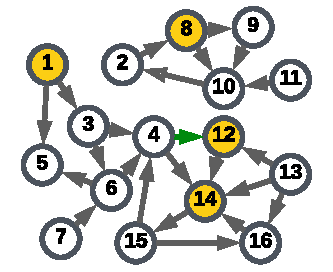
\includegraphics[width=0.23\linewidth]{out/about-frontier-32.pdf}
  }
  \subfigure[After first iteration (DF)]{
    \label{fig:about-frontier-df3}
    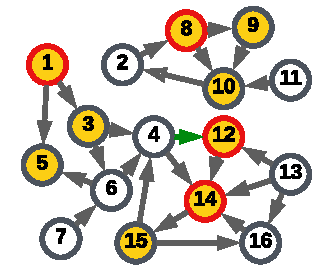
\includegraphics[width=0.23\linewidth]{out/about-frontier-33.pdf}
  }
  \subfigure[After second iteration (DF)]{
    \label{fig:about-frontier-df4}
    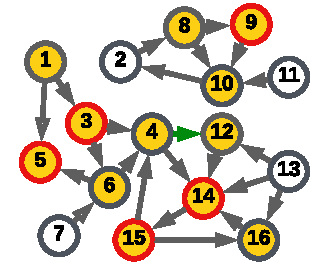
\includegraphics[width=0.23\linewidth]{out/about-frontier-34.pdf}
  } \\[2ex]
  \subfigure[Initial graph]{
    \label{fig:about-frontier-dfp1}
    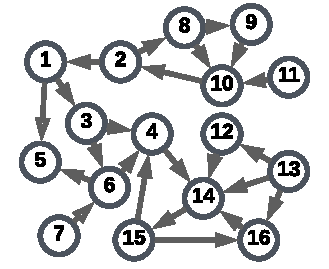
\includegraphics[width=0.23\linewidth]{out/about-frontier-11.pdf}
  }
  \subfigure[Marking initial affected vertices (DF-P)]{
    \label{fig:about-frontier-dfp2}
    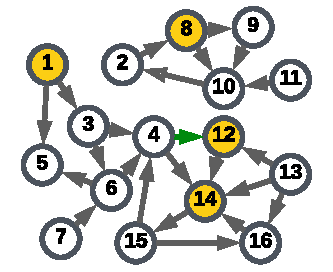
\includegraphics[width=0.23\linewidth]{out/about-frontier-32.pdf}
  }
  \subfigure[After first iteration (DF-P)]{
    \label{fig:about-frontier-dfp3}
    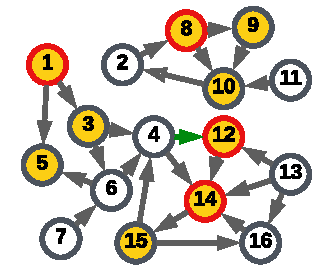
\includegraphics[width=0.23\linewidth]{out/about-frontier-33.pdf}
  }
  \subfigure[After second iteration (DF-P)]{
    \label{fig:about-frontier-dfp4}
    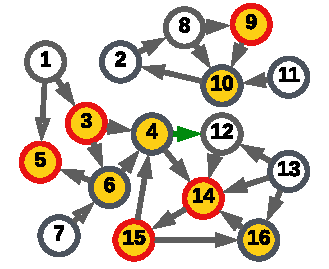
\includegraphics[width=0.23\linewidth]{out/about-frontier-44.pdf}
  } \\[2ex]
  \subfigure[Initial graph]{
    \label{fig:about-frontier-dt1}
    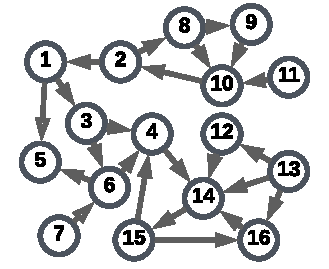
\includegraphics[width=0.23\linewidth]{out/about-frontier-11.pdf}
  }
  \subfigure[Marking affected vertices (DT)]{
    \label{fig:about-frontier-dt2}
    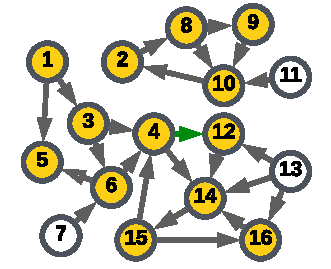
\includegraphics[width=0.23\linewidth]{out/about-frontier-22.pdf}
  }
  \subfigure[After first iteration (DT)]{
    \label{fig:about-frontier-dt3}
    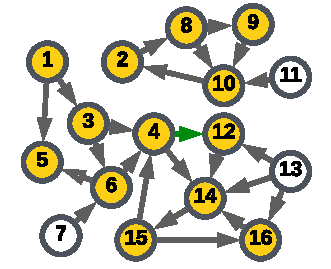
\includegraphics[width=0.23\linewidth]{out/about-frontier-22.pdf}
  }
  \subfigure[After second iteration (DT)]{
    \label{fig:about-frontier-dt4}
    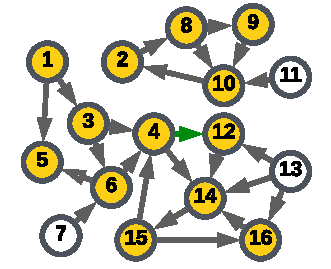
\includegraphics[width=0.23\linewidth]{out/about-frontier-22.pdf}
  } \\[-2ex]
  \caption{An example showcasing our improved \textit{Dynamic Frontier (DF)} and \textit{Dynamic Frontier with Pruning (DF-P)} approaches, in subfigures (a)-(d) and (e)-(h) respectively, in contrast to the \textit{Dynamic Traversal (DT)} approach, shown in subfigures (i)-(l).}
  \label{fig:about-frontier}
\end{figure*}

\ignore{An example showcasing our improved \textit{Dynamic Frontier (DF)} and \textit{Dynamic Frontier with Pruning (DF-P)} approaches. The initial graph has $16$ vertices and $23$ edges. The graph is updated with an edge insertion $(4, 12)$ and an edge deletion $(2, 1)$. Consequently, with DF and DF-P PageRank, the outgoing neighbors of vertices $2$ and $4$ (i.e., vertices $1$, $8$, $12$, and $14$) are marked as affected (shown with yellow fill). In the first iteration, when computing the ranks of these affected vertices, it is observed that the relative change in rank of vertices $1$, $8$, $12$, and $14$ exceeds the frontier tolerance $\tau_f$ (indicated with a red border). Therefore, their outgoing neighbors (i.e., vertices $3$, $5$, $9$, $10$, $14$, and $15$) are also marked as affected, with both DF and DF-P PageRank. In the second iteration, the relative rank change of vertices $3$, $5$, $9$, $14$, and $15$ surpasses the frontier tolerance $\tau_f$, resulting in their outgoing neighbors (i.e., vertices $4$, $6$, $10$, $15$, and $16$) being marked as affected. Additionally, with DF-P PageRank, vertices $1$, $8$, and $12$ are no longer marked as affected as their relative rank change falls below prune tolerance $\tau_p$. In the following iteration, the rankings of affected vertices are updated once more. If the rank change of each vertex falls within the iteration tolerance $\tau$, indicating convergence, the algorithm terminates. In contrast, the \textit{Dynamic Traversal (DT)} approach, marks all vertices reachable from $2$ and $4$ as affected. The ranks of this set of affected vertices are then updated in each iteration.}


\paragraph{Initial marking of affected vertex on edge deletion/insertion:}

For each edge deletion/insertion $(u, v)$, we initially mark the outgoing neighbors of the vertex $u$ in the previous $G^{t-1}$ and current graph snapshot $G^t$ as affected.

\paragraph{Incremental marking of affected vertices upon change in rank of a given vertex:}

Next, while performing PageRank computation, if the rank of any affected vertex $v$ changes in an iteration by an amount greater than the \textit{frontier tolerance} $\tau_f$, we mark its outgoing neighbors as affected. This process of marking vertices continues in every iteration.


\subsubsection{A simple example}

Figure \ref{fig:about-frontier} shows an example of the Dynamic Frontier approach. The initial graph, shown in Figure \ref{fig:about-frontier-01}, comprises $16$ vertices and $25$ edges. Subsequently, Figure \ref{fig:about-frontier-02} shows a batch update applied to the original graph involving the deletion of an edge from vertex $2$ to $1$ and the insertion of an edge from vertex $4$ to $12$. Following the batch update, we perform the initial step of the Dynamic Frontier approach, marking outgoing neighbors of $2$ and $4$ as affected, i.e., $1$, $3$, $4$, $8$, and $12$ are marked as affected (indicated with a yellow fill). Note that vertex $2$ is not affected as it is a source of the change while vertex $4$ being a neighbour of $2$ is marked as affected. Now, we are ready to execute the first iteration of PageRank algorithm.

During the first iteration (see Figure \ref{fig:about-frontier-03}), the ranks of affected vertices are updated. It is observed that the rank changes of vertices $1$ and $12$ surpass the frontier tolerance $\tau_f$ (highlighted with a red border). In response to this, we incrementally mark the outgoing neighbors of $1$ and $12$ as affected, i.e., vertices $3$, $5$, $11$, and $14$. 

During the second iteration (see Figure \ref{fig:about-frontier-04}), the ranks of affected vertices are again updated. Here, its is observed that the change in rank of vertices $3$, $5$, $11$, and $14$ is greater than frontier tolerance $\tau_f$. Thus, we mark the outgoing neighbors of $3$, $5$, $11$, and $14$ as affected, namely vertices $4$, $6$, and $15$. In the subsequent iteration, the ranks of affected vertices are again updated. If the change in rank of each vertex is within iteration tolerance $\tau$, the ranks of vertices have converged, and the algorithm terminates.




\subsection{Synchronous vs Asynchronous implementation}

In a synchronous implementation, separate input and output rank vectors are used, ensuring deterministic results for parallel algorithms through vector swapping at the end of each iteration. In contrast, an asynchronous implementation utilizes a single rank vector, potentially achieving faster convergence and eliminating memory copies for unaffected vertices in dynamic approaches\ignore{, but introduces non-deterministic results in parallel algorithms}.

To assess synchronous and asynchronous implementations for Dynamic Frontier PageRank, both are tested on batch updates (purely edge insertions) ranging from $10^{-7}|E|$ to $0.1|E|$ for Static, Naive-dynamic, Dynamic Traversal, and Dynamic Frontier PageRank. Figure \ref{fig:approach-async} depicts the average relative runtime of asynchronous implementations compared to their synchronous counterparts. Based on the results, we use the asynchronous implementations of Naive-dynamic, Dynamic Traversal, and Dynamic Frontier PageRank --- as they are faster, especially for smaller batch sizes.\ignore{This is due to a somewhat faster convergence and the absence of copy overhead (for Dynamic Traversal and Dynamic Frontier approaches).}




\subsection{Determination of Frontier tolerance ($\tau_f$)}

We now measure a suitable value for frontier tolerance $\tau_f$ that allows us to minimize the number of vertices we process (after marking them as affected), while ensuring that we obtain ranks with the desired tolerance, i.e. we obtain ranks with no higher error than Static PageRank for the same tolerance setting. For this, we adjust frontier tolerance $\tau_f$ from $\tau$ to $\tau / 10^5$ and obtain ranks of vertices with the Dynamic Frontier approach on batch updates (consisting purely of edge insertions) of size $10^{-7}|E|$ to $0.1|E|$.

Figure \ref{fig:adjust-frontier} illustrates the average relative runtime and rank error (in comparison to ranks obtained with reference Static PageRank) using the Dynamic Frontier approach. The figure suggests that as $\tau_f$ increases, runtime decreases, but it is accompanied by an increase in error. A frontier tolerance $\tau_f$ set at $\tau/10^4$ or $\tau/10^5$ yields ranks with lower error than Static PageRank, making them acceptable for uniformly random batch updates. To err on the side of caution, we opt for a frontier tolerance of $\tau_f = \tau/10^5$.

\begin{figure*}[!hbt]
  \centering
  \subfigure[Speedup with varying Frontier tolerance $\tau_f$]{
    \label{fig:adjust-frontier--speedup}
    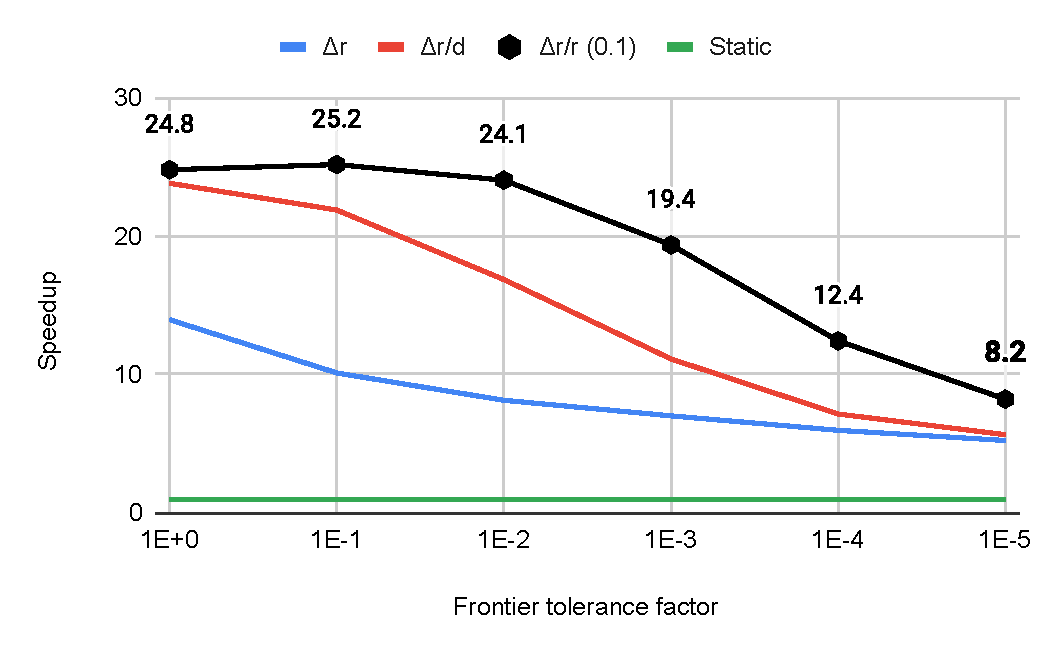
\includegraphics[width=0.48\linewidth]{out/adjust-frontier-speedup.pdf}
  }
  \subfigure[Error in ranks obtained with varying Frontier tolerance $\tau_f$]{
    \label{fig:adjust-frontier--error}
    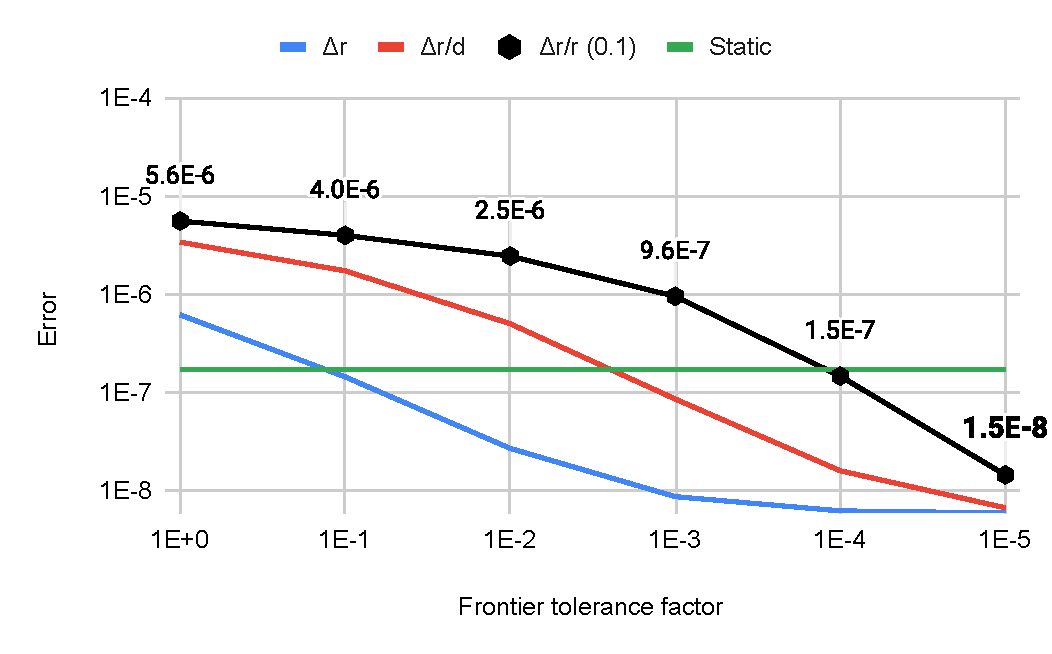
\includegraphics[width=0.48\linewidth]{out/adjust-frontier-error.pdf}
  } \\[-2ex]
  \caption{Average Speedup and Error in ranks obtained (with respect to ranks obtained with Reference Static PageRank) using \textit{Dynamic Frontier} approach, with frontier tolerance $\tau_f$ varying from $\tau$ to $\tau / 10^5$, on batch updates of size $10^{-7}|E|$ to $0.1|E|$. The figures indicate that increasing $\tau_f$ reduces runtime, but also increases the error. A Frontier tolerance $\tau_f$ of $\tau/10^4$ and $\tau/10^5$ obtain ranks with error lower than \textit{Static} PageRank, and are thus acceptable (we choose $\tau_f = \tau/10^5$ to be on the safe side).}
  \label{fig:adjust-frontier}
\end{figure*}

\begin{figure*}[!hbt]
  \centering
  \subfigure{
    \label{fig:adjust-prune--speedup}
    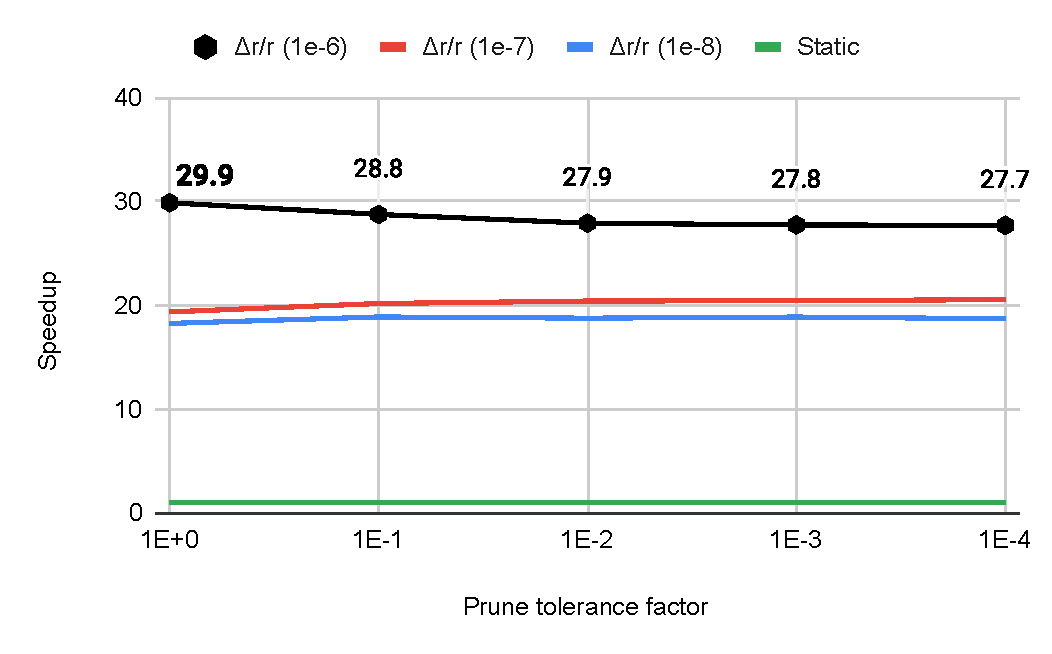
\includegraphics[width=0.48\linewidth]{out/adjust-prune-speedup.pdf}
  }
  \subfigure{
    \label{fig:adjust-prune--error}
    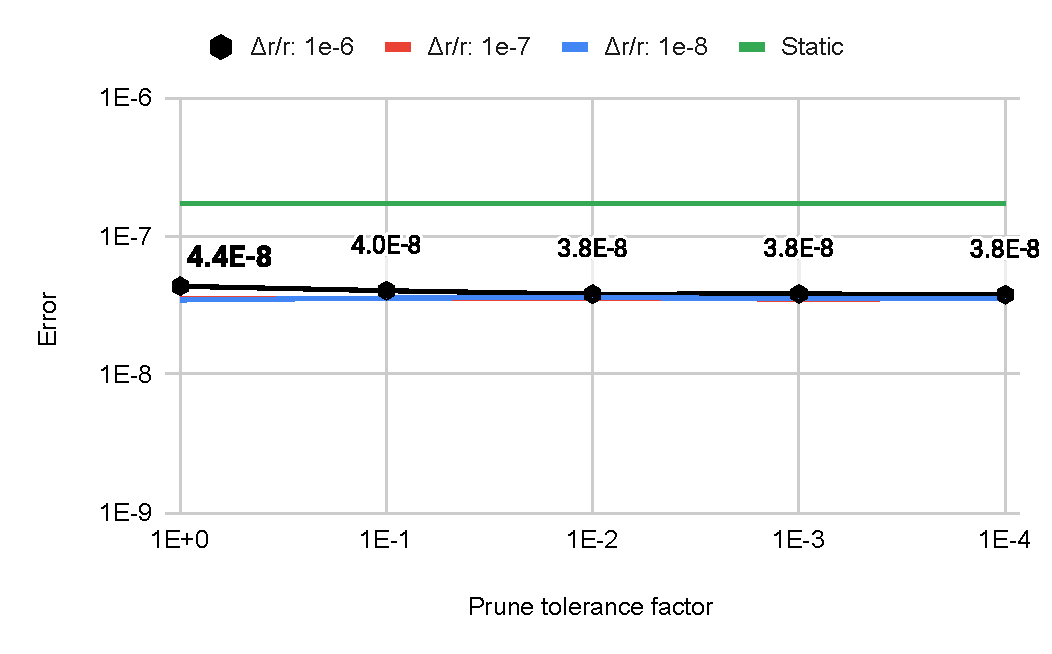
\includegraphics[width=0.48\linewidth]{out/adjust-prune-error.pdf}
  } \\[-2ex]
  \caption{Average Relative runtime with asynchronous implementations of \textit{Static}, \textit{Naive-dynamic}, \textit{Dynamic Traversal}, and \textit{Dynamic Frontier} approach compared to their respective synchronous implementations, on batch updates of size $10^{-7}|E|$ to $0.1|E|$ (right), and overall (left). The results indicate that asynchronous implementations are faster than synchronous ones, especially for smaller batch sizes. This is due to a somewhat faster convergence and the absence of copy overhead (for \textit{Dynamic Traversal} and \textit{Dynamic Frontier} approaches).}
  \label{fig:adjust-prune}
\end{figure*}

\begin{algorithm}[!hbt]
\caption{Our parallel Dynamic Frontier (DF) PageRank.}
\label{alg:frontier}
\begin{algorithmic}[1]
\Require{$G^{t-1}, G^t$: Previous, current input graph}
\Require{$\Delta^{t-}, \Delta^{t+}$: Edge deletions and insertions (input)}
\Require{$R^{t-1}, R$: Previous, current rank vector}
\Ensure{$\Delta r$: Change in rank of a vertex}
\Ensure{$\Delta R$: $L\infty$-norm between previous and current ranks}
\Ensure{$\tau, \tau_f, \tau_p$: Iteration, frontier, prune tolerance}
\Ensure{$\alpha$: Damping factor}

\Statex

\Function{dynamicFrontier}{$G^{t-1}, G^t, \Delta^{t-}, \Delta^{t+}, R^{t-1}$}
  \State $R \gets R^{t-1}$ \label{alg:frontier--initialize}
  \State $\rhd$ Mark initial affected
  \ForAll{$(u, v) \in \Delta^{t-} \cup \Delta^{t+} \textbf{in parallel}$} \label{alg:frontier--mark-begin}
    \ForAll{$v' \in (G^{t-1} \cup G^t).out(u)$}
    \State Mark $v'$ as affected
    \EndFor
  \EndFor \label{alg:frontier--mark-end}
  \ForAll{$i \in [0 .. MAX\_ITERATIONS)$} \label{alg:frontier--compute-begin}
    \State $\Delta R \gets 0$
    \ForAll{affected $v \in V^t$ \textbf{in parallel}}
      \State $r \gets (1 - \alpha)/|V^t|$
      \ForAll{$u \in G^t.in(v)$}
        \State $r \gets r + \alpha * R[u] / |G^t.out(u)|$
      \EndFor
      \State $\Delta r \gets |r - R[v]|$ \textbf{;} $\Delta R \gets \max(\Delta R, \Delta r)$
      \State $\rhd$ Prune $v$ if its relative rank change is small
      \If{$\Delta r / \max(r, R[v]) \leq \tau_p$}
        \State Mark $v$ as not affected
      \EndIf
      \State $\rhd$ Expand frontier if relative rank change is large
      \If{$\Delta r / \max(r, R[v]) > \tau_f$} \label{alg:frontier--remark-begin}
        \ForAll{$v' \in G^t.out(v)$}
          \State Mark $v'$ as affected
        \EndFor
      \EndIf \label{alg:frontier--remark-end}
      \State $\rhd$ Update rank of $v$
      \State $R[v] \gets r$
    \EndFor
    \State $\rhd$ Ranks converged?
    \If{$\Delta R \le \tau$} \textbf{break}
    \EndIf
  \EndFor \label{alg:frontier--compute-end}
  \State \ReturnInline{$R$} \label{alg:frontier--return}
\EndFunction
\end{algorithmic}
\end{algorithm}




%% Requires (parameters):
% G(V, E): a directed unweighted graph
% R: initial ranks (1/N for static)

%% Parameter values:
% MAX\_ITERATIONS = 500
% DAMPING\_FACTOR = 0.85
% TOLERANCE = 10^-10





\subsection{Our Dynamic Frontier PageRank implementation}

Algorithm \ref{alg:frontier} shows our implementation of Dynamic Frontier PageRank, which is designed to compute the PageRank of vertices in a graph while efficiently handling dynamic changes in the graph structure over time. The algorithm takes as input the previous and current versions of the graph, edge deletions and insertions in the batch update, and the previous rank vector.

It begins by marking the initially affected vertices based on the edge deletions $\Delta^{t-}$ and insertions $\Delta^{t+}$ in parallel (lines \ref{alg:frontier--mark-begin}-\ref{alg:frontier--mark-end}). It then enters an iterative computation phase (lines \ref{alg:frontier--compute-begin}-\ref{alg:frontier--compute-end}), where it updates the rank of each affected vertex. The PageRank computation is performed in parallel for each affected vertex $v$, considering the incoming edges $G^t.in(v)$. The algorithm checks whether the change in rank $\Delta r$ exceeds the frontier tolerance $\tau_f$, and marks its out-neighbor vertices as affected if so. The iteration continues until either the net change in ranks $\Delta R$ (which is equal to the $L\infty$-norm between the previous and the current ranks) falls below the iteration tolerance $\tau$, or a maximum number of iterations is reached $MAX\_ITERATIONS$. In line \ref{alg:frontier--return}, the final rank vector $R$ is returned.




% Dynamic Frontier (DF) approach
% Adjusting tolerance, Frontier tolerance, Mark DelRank / DelContrib
% Dynamic Frontier optimizations
% Edge-balanced approach (Chunk size)
